\chapter{Methods}
In this chapter we review the basic implementation details of our ViDA
framework. We first demonstrate how we use Lucas-Kanade and Farneback optical
flow algorithms to reduce the feature space to only six 25 bin feature vectors.
With that feature space, we outline how to classify the videos using several
well known machine learning algorithms such as K-nearest neighbors and support
vector machines (SVM). Finally, we cover how we designed this system to be
completely horizontally and vertically scalable on the AWS cloud.


\section{\label{section} Implementing Optical Flow in ViDA}
In our software, we use two OpenCV library calls, \texttt{goodFeaturesToTrack}
and \\
\texttt{calcOpticalFlowPyrLK} to implement the Lucase-Kanade Pyrmidal optical
flow. The first function is used to find features that can be easily tracked
from one frame to the other using the Shi-Tomasi algorithm \cite{shi1994good}.
The next method then calculates the optical flow between the good points using
the pyramidal implementation of the Lucas-Kanade algorithm
\cite{bouguet2001pyramidal}. Algorithm \ref{alg:lk_flow} outlines the general
program flow for calculating motion vectors in ViDA.

\begin{algorithm}
\caption{Calculating Lucas-Optical Flow from Videos}
\label{alg:lk_flow}
\begin{algorithmic}[1]
\Procedure{CalculateVectors}{$frame1$, $frame2$}
  \If{\text{$track\_points\_initialized$}}
  	\State $opticalflow \gets \texttt{calcOpticalFlowPyrLK}(track\_points, frame1, frame2)$
  \Else
  	\State $track\_points \gets \texttt{goodFeaturesToTrack}(frame1)$
	\State $track\_points\_initialized \gets True$
	\State $optical\_flow \gets  \texttt{CalculateVectors}(frame1, frame2)$
  \EndIf
  \Return $optical\_flow$
\EndProcedure
\end{algorithmic}
\end{algorithm}

The algorithm used in ViDA is similar to Algorithm \ref{alg:lk_flow} but
contains fewer steps since there is no need to get good features to track.
In the C++ software, we also implemented Farneback method. The
Farneback implementation is shown in Algorithm \ref{alg:farneback}.

\begin{algorithm}
\caption{Calculating Farneback Flow from Videos}
\label{alg:farneback}
\begin{algorithmic}[1]
\Procedure{CalculateVectors}{$frame1$, $frame2$}
  \State $optical\_flow \gets \texttt{calcOpticalFlowFarneback}(frame1, frame2)$\\
  \Return $optical\_flow$
\EndProcedure
\end{algorithmic}
\end{algorithm}

As can be seen in \ref{alg:farneback}, we don't need any good features to track
because we are calculating the optical flow globally between frames, rather than
selecting a few features. This has the advantage of tracking optical flow objects
that may fail the Shi-Tomasi method for tracking, but because it is no discriminant
in the features, the resulting motion vectors are dense.


\section{\label{section:comparison}Comparison of Methods}
We implemented the Lucas-Kanade method first in our research because in general,
performance is a concern and, as long as not too many features or
too few features are detected, the Lucas-Kanade algorithm will be faster
\cite{de2015choosing}. Despite this fact, we found that our classifier did
not perform as well on features extracted from the Lucas-Kanade method, as it
did using the Farneback method. Hence most of the results in this thesis
have been calculated with Farneback optical flow unless otherwise specified.

\section{\label{section:feature_extraction}Feature Extraction from Optical Flow}
The \texttt{CalculateVectors} function in both Algorithm \ref{alg:lk_flow} and
\ref{alg:farneback} returns several dense matrices that represent the features
that we can extract from the optical flow output. These features are magnitude,
orientation, x direction and y direction of the optical flow features. These are
ultimately the features that we use to train and classify using an SVM. However,
if we had two $N \times M$ video frames as the input, we now have $4 \times N
\times M$ features. Clearly we have not yet reduced the input feature space.
Thus, based on information that we know \textit{a-priori}, we can reduce our
feature space significantly.

In the case of typing and writing, we know we can expect there to be motion from
one frame to the next. We don't know by how much, but we do know that it is not
zero. Using this knowledge, we can then threshold the optical flow vectors that
we get back from Algorithms \ref{alg:lk_flow} and \ref{alg:farneback}. The
threshold value used was empirically calculated from doing multiple runs on the
AOLME videos. We found we got the best results by only retrieving
optical flow vectors with a magnitude greater than 75\% of the max value. The set
of Equations in \ref{eq:optical_threshold} illustrate this idea.

\begin{align}
  \label{eq:optical_threshold}
  \begin{split}
  \mathbf{V} &= (\mathbf{V_x}, \mathbf{V_y}) \\
  \mathbf{V_m} &=
  \begin{cases}
    1, & \text{if } \|\mathbf{V}\| \geq \max( \|\mathbf{V}\|) \times 0.25 \\
    0, & \text{otherwise}
  \end{cases}
  \end{split}
\end{align}

where $\mathbf{V_x}$ and $\mathbf{V_y}$ are the optical flow vectors in the
x and y directions respectively. $\mathbf{V_m}$ is the bit mask that is
then used to extract the subset of data from each of the dense matrices.

\begin{align}
  \label{eq:subset}
  \begin{split}
  \text{Let: } \\
  \|\mathbf{V\prime}\| &= \|\mathbf{V}\| \circ \mathbf{V_m}\\
  \mathbf{V_x\prime} &= \mathbf{V_x} \circ \mathbf{V_m}\\
  \mathbf{V_y\prime} &= \mathbf{V_y} \circ \mathbf{V_m}\\
  \mathbf{\Phi\prime} &= \mathbf{\Phi} \circ \mathbf{V_m}
\end{split}
\end{align}

Using the optical flow bitmask, $\mathbf{V_m}$, we can then extract features
from each one of our dense matrices using the Hadamard product as shown in
Equation \ref{eq:subset}, where $\|\mathbf{V\prime}\|,
\mathbf{V_x\prime},\mathbf{V_y\prime}, \mathbf{\Phi\prime}$ are subset matrices
for the magnitude, x and y direction and orientation respectively. We have now
reduced the feature space somewhat, but depending on the size of the video and the
amount of entropy per frame pair, we could still have a significant amount of
data to process for classification, this idea is especially true for
Farneback optical flow.

In addition to extracting generic vectors from the video, we also add
geometrical centroids, blob orientation and background motion around the blobs
to the optical flow statistics being used for classification. We implement these
methods to attempt to leverage information that could be useful during
classification. In order to calculate the geometrical centroids and orientations
of each blob, we use some well known algorithms available in OpenCV,
\texttt{connectedComponentsWithStats} and \texttt{findContours}
\cite{itseez2015opencv}. \texttt{connectedComponentsWithStats} is a function
that allows us to compute the centroid for each blob of connected pixels. The
input to this function is our binary mask image, $\mathbf{V_m}$. Once we have
all the connected blobs, we can then calculate the orientation of each one of
those blobs using \texttt{findContours} in combination with with
\texttt{fitEllipse}. The full implementation of this algorithm is outlined in
Appendix \ref{ap:centroids}. The final step is to then dilate each blob, and
then retrieve the magnitude of the optical flow in this region. Appendix
\ref{ap:dilate}. Figure \ref{fig:orient_cent} illustrates the idea of acquiring
the centroid and orientation of the blobs from $\mathbf{V_m}$.

\begin{figure}[h]
  \label{fig:orient_cent}
  \centering
  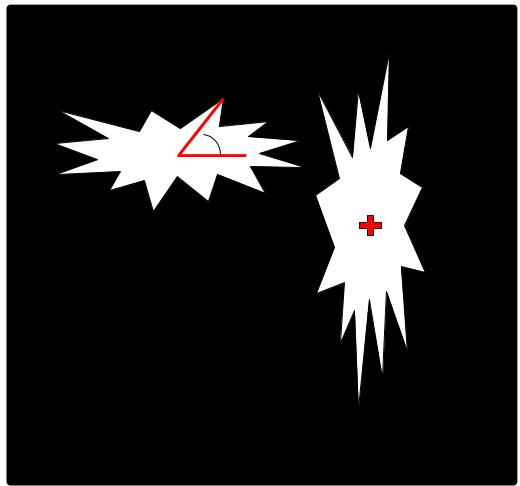
\includegraphics[width=8cm]{figures/cent_and_orient}
  \caption{Example of orientation measurement on the left, and the centroid
  calculation on the right.}
\end{figure}

When the previous optical flow features have been generated, their values are
then organized into a probability density function (PDF) with 25 bins. That is
to say that each frame pair generates a PDF and that PDF is accumulated for
every subsequent frame in the video sequence. When our software reaches the end
of the video file, a normalized, cumulative distribution function (CDF) is
calculated and output for each vector. So for each input video there will be one
CDF with 25 bins for blob orientation, blob centroid x and y, motion vector
magnitude, motion vector orientation and background motion vector magnitude.
Figure \ref{fig:extract_flow} clearly illustrates this concept.

\begin{figure}[h]
  \label{fig:extract_flow}
  \centering
  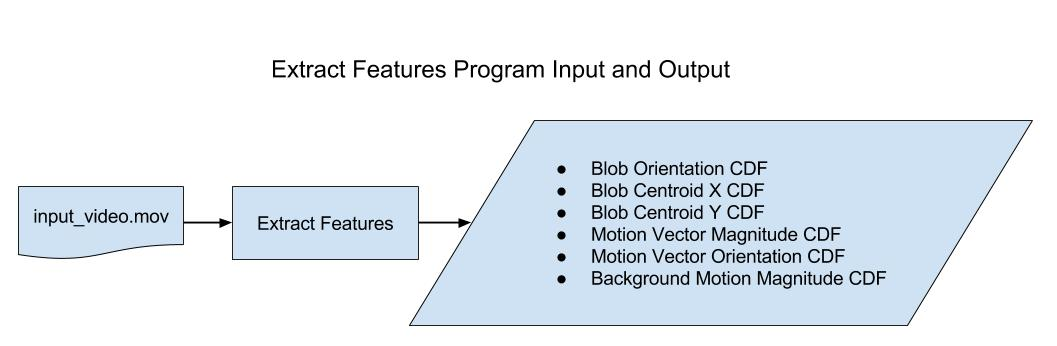
\includegraphics[width=14cm]{figures/extract_features_flow}
  \caption{Flow of the extract features program. For every input video, it will
  return a CDF with 25 bins for each of the extracted features from the motion
  vectors}
\end{figure}

Ultimately, these are the features that are then accumulated for multiple AOLME
videos and used for classification.

\section{\label{section:classification}Classifying the Reduced Feature Space}
At this point we now have accumulated a bag of features for videos. The features
that are collected are stored in a comma separated file (csv) that can be read
in by the any of the popular machine learning packages such as those provided
by the R language or Python's SciKit-Learn. The file contains labels that have
filename, centroid x CDF, centroid Y CDF, background motion CDF, motion magnitude
CDF, motion orientation CDF and classification. We can then use an SVM to classify
the features. To validate our results, we use leave-one-out cross validation
to ensure that we have not overfit the data.

\section{\label{section:distributed_processing}Scalable Architecture}
A core principal for a well designed, horizontally scalable application, is
to design it such that it does not contain state \cite{awsbestpractices}.
When state is required, it the software complexity increases substantially and
makes it difficult to distribute the system over a scalable amount of nodes.
However, if the software was designed such that each service can operate and
stand on its own, it is the perfect embarrassingly parallel computing task to
tackle. For this thesis we focus on ensuring that our feature extractor,
as described in Section \ref{section:feature_extraction}, is completely stateless.
This is a design feature that has allowed us the flexibility to scale our
system over as many nodes as are available on the AWS cloud.

\subsection{\label{subsection:architecture_overview}Architecture Overview}
Our system builds upon AWS to create an easy-to-maintain and easy-to-scale
video processing system. We use S3 storage to put small video clips that
have been extracted from our AOLME dataset. These clips are made available to
to all of the processing nodes. The processing nodes communicate with the master
node using Amazon's simple queue service (SQS). Figure \ref{fig:dataflow} illustrates
the basic distributed system design.

\begin{figure}[h]
  \label{fig:dataflow}
  \centering
  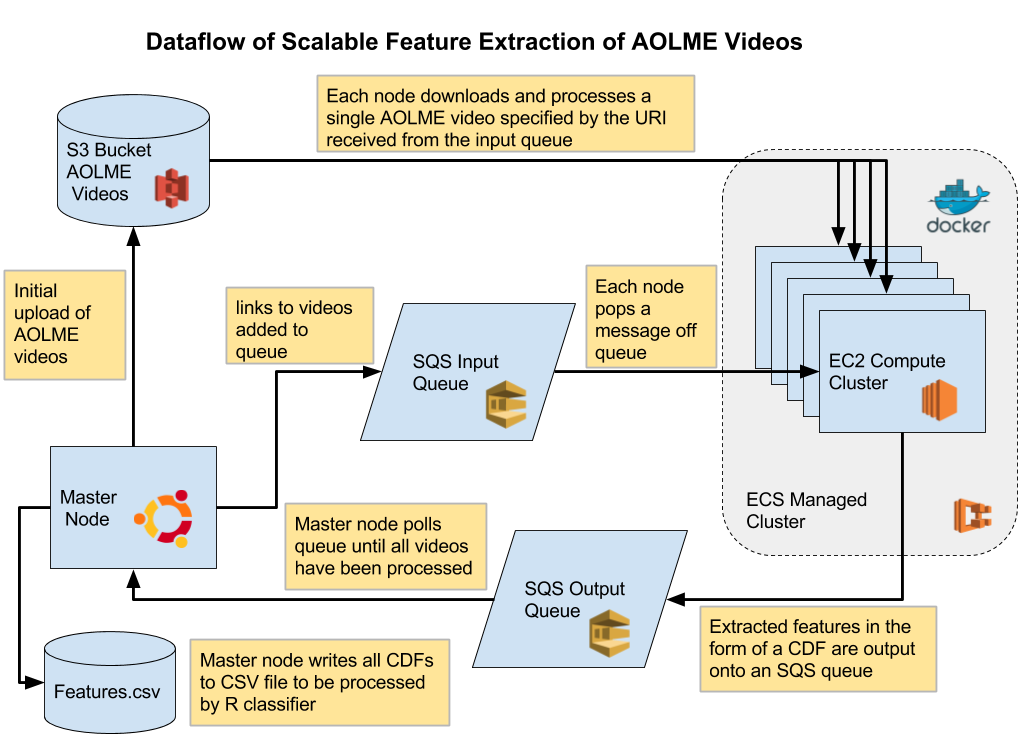
\includegraphics[width=\textwidth]{figures/extract_features_dataflow}
  \caption{Dataflow of the distributed video system using AWS components}
\end{figure}

From Figure \ref{fig:dataflow} we see that the first step is to upload
the videos to S3. We keep the videos very small, because as we show in our experiments
section, it takes quit a long time to process large videos therefore there is a
significant benefit to keeping the video chunks relatively small so that many
machines could potentially work on the feature extraction process. The next step
is to place a message on the SQS queue specifying which video to process and
what its classification is. For the purposes of this thesis, we manually place
messages on the queue so that we can control the flow of messages. In
a production system though, we would have the S3 bucket notify the SQS queue that
a new video was uploaded and ready for processing. The third step is the processing
step. In our setup, we create 20 EC2 instances running our feature extractor application.
Each one of these instances polls the SQS queue waiting for a message to arrive.
As soon as one does, it downloads the appropriate video from the S3 bucket,
processes the video, and then places the results on another SQS queue. At this
point, the master node is polling the results queue and collecting the results
into a csv file. Finally, the csv file can be used to train the SVM in the R
code.

\subsection{\label{subsection:master_node}Master Node Configuration}
The master node in our system is responsible for sending out jobs to process and
then coalescing the results from the calculations performed by the slave nodes.
All of these processes are done using the boto3 \cite{boto3} Python  software
development kit (SDK). The core implementation of AWS uses a  representational
state transfer like (RESTful) interface to communicate to all the services that
Amazon offers in a programatic  way, but they also offer several easy-to-use
object oriented libraries written  in several languages to make programming easier
for the end user. The master node
need not be any specific operating system as long as the Python language
can be interpreted on it. In this thesis, we use Ubuntu 14.04 to run our master
node logic, but it could just as well be OS x or any other flavor of linux.

The master node performs several basic tasks. The first of which is to put
messages on the SQS queue.  This is orchestrated by reading
a csv file that consists of an S3 link to a video segment, the classification of
the segment, the SQS queue to which to output the features and finally the
optical flow method to use. An example of the file is show in Table
 \ref{table:message_queue}.

\begin{table}[h]
  \label{table:message_queue}
  \begin{tabular}{ | l | l | l | p{3cm} |}
  \hline
  \textbf{path} & \textbf{classification} & \textbf{sqs\_queue} & \textbf{of\_algorithm}\\ \hline
  aolme/data/typing/seg\_1.mp4 & 1 & feature\_queue & farneback \\ \hline
  aolme/data/notyping/seg\_1.mp4 & 2 & feature\_queue & farneback \\
  \hline
  \end{tabular}
  \caption{Example of data file that use by the master node to place messages on
  the SQS queue. }
\end{table}

From the example data shown in Table \ref{table:message_queue}, we can see that
the nodes have the ability to switch the algorithm as well as associate a
classification from the video. Having the ability to switch method types allows
us to easily benchmark using Lucas-Kanade optical flow versus Farneback.
We also put the output queue in the message so that the slave nodes know to which
queue to place the results of their calculations. This information is also necessary
for the master to know which queue to wait on to collect all the results. Additionally,
if we need more information to be passed to the slave nodes so that they can
effectively do their job, we can easily put that information in the queue with
the message trivially.

Once the master node has sent all the messages to the queue, it then polls
on the queue it placed the messages on to verify that all the messages have been
remove by the slave nodes. This is an important step to validate that the
slave nodes are indeed popping messages off the SQS queue and processing
the videos that are associated with each message. Once this has been validated,
the master node begins to poll on the designated output queue for the results output
from each of the slave nodes. Once all the results have been collected, the master
node places each of the vectors into a comma separated features file.
The pseudo code for the operations performed by the master are show in Algorithm
\ref{alg:master_node}.

\begin{algorithm}
\caption{Master Node Implementation Pseudo-Code}
\label{alg:master_node}
\begin{algorithmic}[1]
  \State $videos\_to\_process \gets \texttt{ReadInputData(input.csv)}$
  \For{\texttt{i = 0; i < len(videos\_to\_process); ++i}}
    \State $sqs\_message \gets \texttt{CreateMessage(videos\_to\_process[i])}$
    \State $output\_queue\_uri \gets videos\_to\_process[i].output\_queue\_uri$
    \State$\texttt{SendSqsMessage(}sqs\_message, sqs\_uri \texttt{)}$
  \EndFor

  \While{$\texttt{MessagesRemainingInQueue(}sqs\_uri \texttt{)} \neq 0$} \Comment{Poll queue every second}
    \State $\texttt{Sleep(1)}$
  \EndWhile

  \While{$\texttt{MessagesRemainingInQueue(}output\_queue\_uri\texttt{)} \neq 0$}
    \State $feature\_vectors \gets \texttt{ReceiveSqsMessage(output\_queue\_uri\texttt{)}}$
    \State $\texttt{Sleep(1)}$
  \EndWhile

  \State \texttt{WriteFeaturesToDisk(} $feature\_vectors$ \texttt{)}

\end{algorithmic}
\end{algorithm}
